%%%%%%%%%%%%%%%%%%%%%%%%%%%%%%%%%%%%%%%%%%%%%%%%%%%%%%%%
\fondo{celeste}
\section{Introducción}
\fondo{blanco}
%%%%%%%%%%%%%%%%%%%%%%%%%%%%%%%%%%%%%%%%%%%%%%%%%%%%%%%%

%%%%%%%%%%%%%%%%%%%%%%%%%%%%%%%%%%%%%%%%%%%%%%%%%%%%%%%%
\begin{frame}
    \begin{columns}
    \column{.6\textwidth}
    \begin{block}{}\centering\Large
        ¿Pedir a los estudiantes que lean un capítulo antes de la clase es realmente aula invertida?
    \end{block}      
    \column{.4\textwidth}
        \begin{center}
        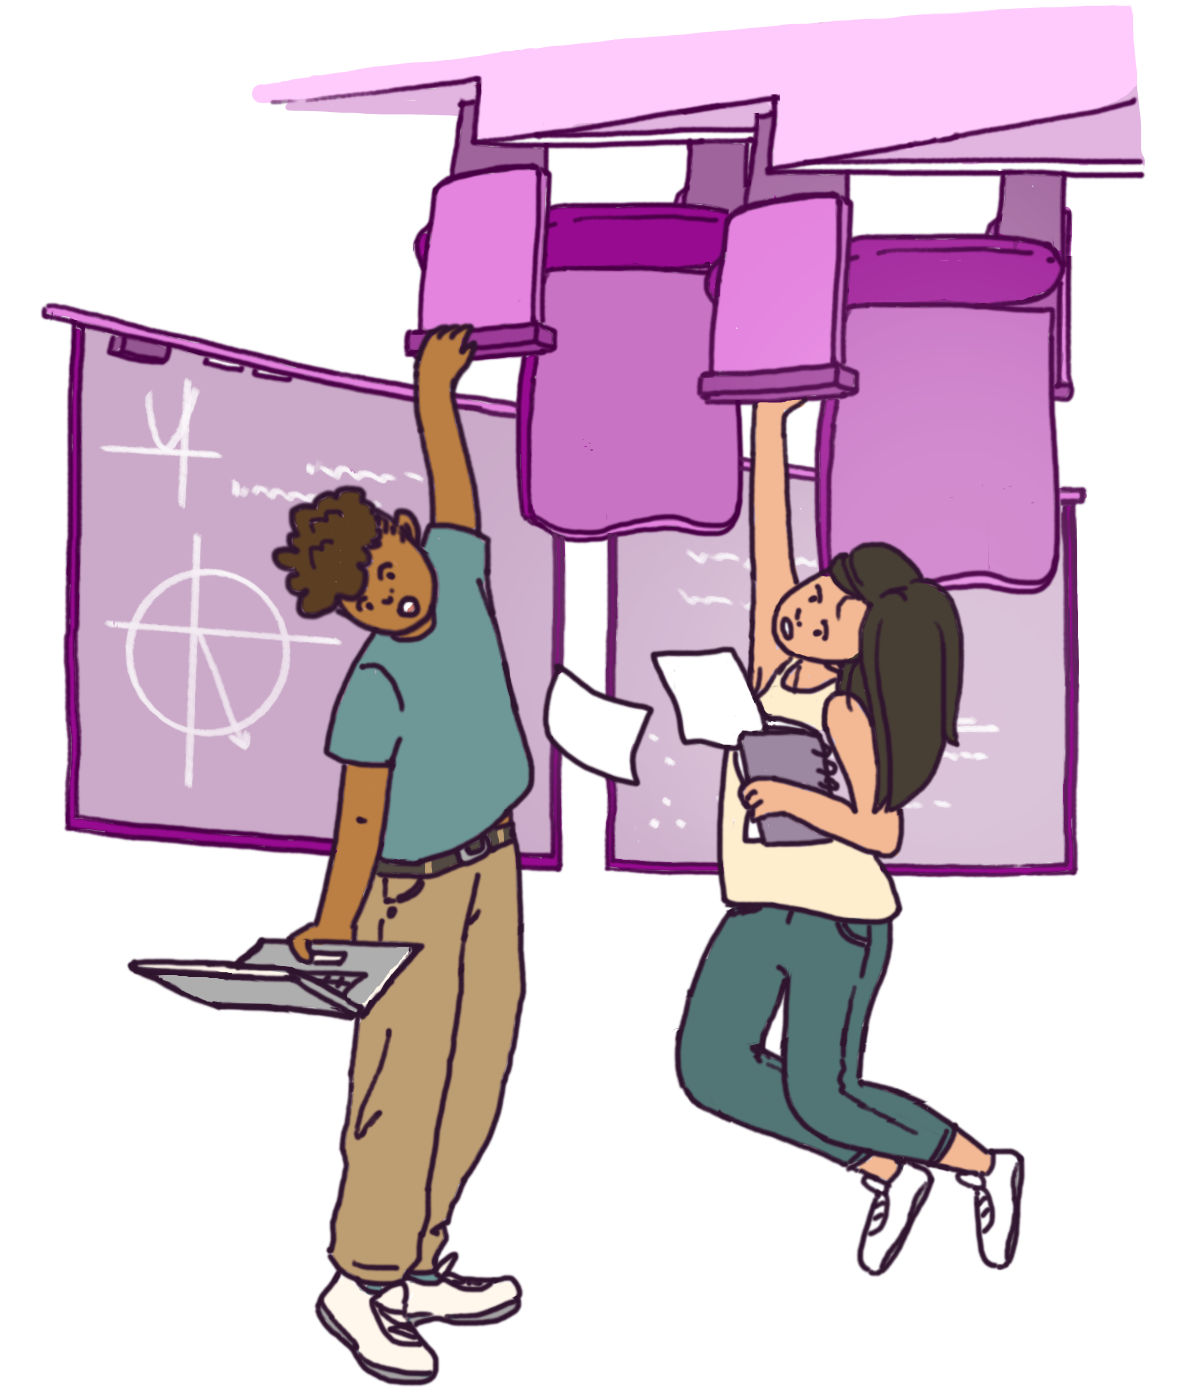
\includegraphics[width=1\linewidth]{Figuras/Fig01.png}
        \end{center}
    \end{columns}

\end{frame}

%%%%%%%%%%%%%%%%%%%%%%%%%%%%%%%%%%%%%%%%%%%%%%%%%%%%%%%%
\begin{frame}
    \begin{block}{Objetivo de la charla}
        \begin{itemize}[leftmargin=*]
            \item Presentar la metodología para integrar ChatGPT en el aula invertida.
            \item Motivar a replicar esta experiencia en otras asignaturas o contextos.
        \end{itemize}
    \end{block}

    \vspace{0.3cm}
    \pause
    \begin{block}{}\centering
        Caso de uso: Álgebra Lineal
    \end{block}
\end{frame}

